\subsection{Gran Breta\~na}
En esta instancia de experimentaci'on vamos a analizar las rutas a la universidad de Oxford, ubicada en Inglaterra, utilizando la direcci'on \textit{ox.ac.uk}. 
El origen del mensaje es una direcci'on en Argentina y en un principio esperamos, basados en los mapas de cables submarinos, ver 2 o m'as saltos intercontinentales. Si bien
existen caminos con 2 saltos intercontinentales, podria ser 3 si una ruta pasa por europa continental. 

Utilizando 30 repeticiones por cada \textit{TTL}  conseguimos los siguientes datos hasta que el mensaje llego a su destino.

\begin{tabular}{ |p{1cm}||p{3cm}|p{2cm}|p{2cm}|p{1.5cm}|  }
 \hline
 \multicolumn{5}{|c|}{Traceroute a Oxford} \\
 \hline
 \textit{TTL} & \textit{IP}  & \textit{RTT} & $\delta$\textit{RTT} & Outlier? \\
 \hline
 1   & 192.168.1.1   & 2.08 ms &   - &   \\
 2   & Sin respuesta  & - 	&   - &   \\
 3   & Sin respuesta  & - 	&   - &   \\
 4   & Sin respuesta  & - 	&   - &   \\
 5   & Sin respuesta  & - 	&   - &   \\
 6   & 200.89.161.77  & 31.76 ms &  29.67 ms &   \\
 7   & 200.89.165.197  & 36.68 ms &  4.93 ms &    \\
 8   & 200.89.165.222  & 33.3 ms &  - &   \\
 9   & Sin respuesta  & - &   - &   \\
 10   & 67.17.94.249 & 165.04 ms &  131.74 ms & Outlier \\
 11   & Sin respuesta   & - &   - &   \\
 12   & Sin respuesta   & - &   - &   \\
13   &   212.187.139.166&    238.81 ms  &      73.77 ms  & Outlier  \\    
14   &   146.97.35.197  &    246.8 ms   &      7.99 ms  &   \\       
15   &   146.97.33.2   &     243.96 ms  &      -    &   \\         
16   &   146.97.37.194   &   250.65 ms  &      6.69 ms  &    \\       
17   &   193.63.108.94   &   243.61 ms  &      -   &    \\         
18    &  193.63.108.98   &   247.05 ms    &     3.44 ms   &    \\       
19   &   193.63.109.90  &    248.58 ms  &      1.53 ms  &     \\
20   &   Sin respuesta              &    -          &      -    &   \\   
21   &   192.76.32.66   &    245.76 ms  &      -     &   \\    
22   &   129.67.242.154  &   223.77 ms   &     -   &   \\
 \hline
\end{tabular}

\smallskip

Los paquetes con \textit{TTL} 1 a 4 y 11 a 12  no responden con un mensaje de error que nos permita detectarlos.
Creemos que es porque son dispositivos dentro de la red de los proveedores locales de internet que priorizan otras tareas y deciden no
responder con un mensaje utilizando sus recursos m'as eficientemente. Algunos saltos pueden ser dispositivos optimizados para ciertas tareas
las cuales no incluyen responder a \textit{TTL} excedidos o bien deciden no hacerlo para optimizar trafico. 

Multiples saltos mostraron una anomalia com'un donde \textit{TTL} $i$ es menor a \textit{TTL} $i-1$, es decir que un mensaje tardo menos en hacer $i$ saltos
que $i-1$ saltos lo cual no tiene ning'un sentido. Esto se puede explicar por las diferentes capacidades y trafico actual de los enlaces o tal vez por
la ruta elegida para enviar el mensaje de error. En estos casos ignoramos esos saltos en el analisis. \\

Nuestro programa logr'o detectar 2 saltos intercontinentales en \textit{TTL} 10 y \textit{TTL} 13, correspondientes al un salto entre Argentina y Estados Unidos y
entre Estados Unidos e Inglaterra correspondientemente.
Podemos ver esto con el siguiente grafico que muestra los saltos con sus respectivas IPs y los tiempos (RTT y RTT normalizados a $N(0,1)$ con el l'imite
utilizado para detectar outliers.

\begin{figure}[H]
\centering
\caption{Oxford delta RTTs y ZRTT}
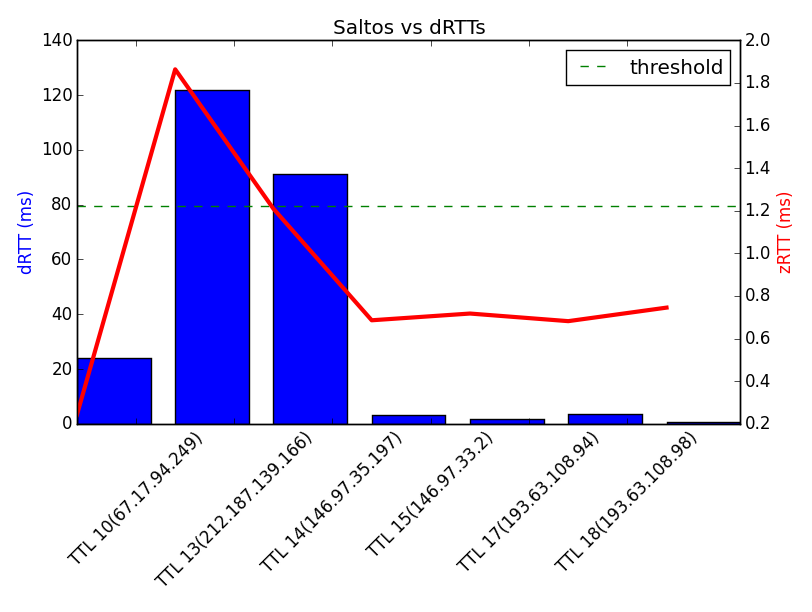
\includegraphics[width=0.55\textwidth]{modules/oxford_rtts_2}
 \label{fig:oxford_rtts_2}
\end{figure}

Los caminos encontrados no dieron mucho lugar a calculos de deltas por la anomalia descripta lo cual se puede ver graficamente en la siguiente figura
\begin{figure}[H]
\centering
\caption{Oxford RTTs por salto}
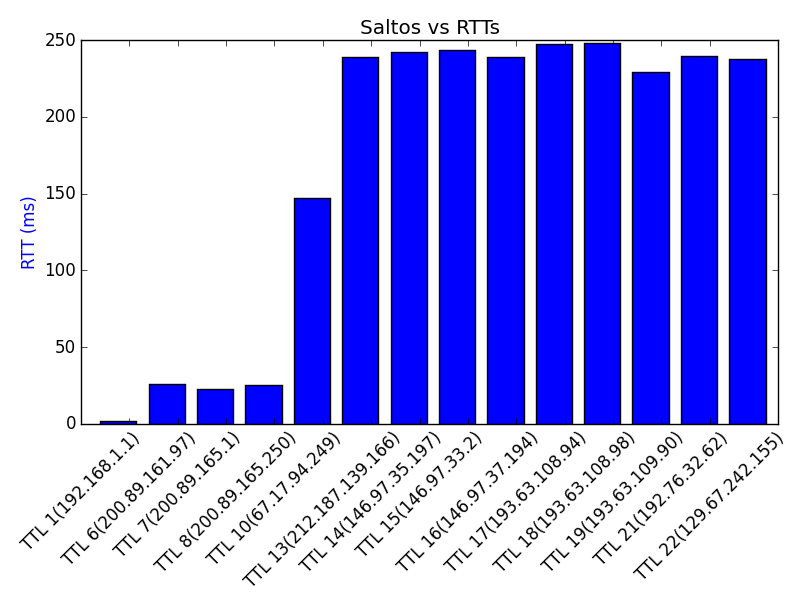
\includegraphics[width=0.55\textwidth]{modules/oxford_rtts_1}
 \label{fig:oxford_rtts}
\end{figure}


En el siguiente gr'afico podemos ver el camino completo que el mensaje recorri'o para llegar a su destino en Oxford. Paso por Estados Unidos y luego directo a 
Inglaterra. Nuestro software no logra detectar este enlace como intercontinental, en la gran mayoria de las pruebas el l'imite impuesto por el algoritmo de
Cimbala esta muy cerca de los valores de \textit{RTT} pero no logran pasarlo.
\begin{figure}[H]
\centering
\caption{Ruta a Oxford}
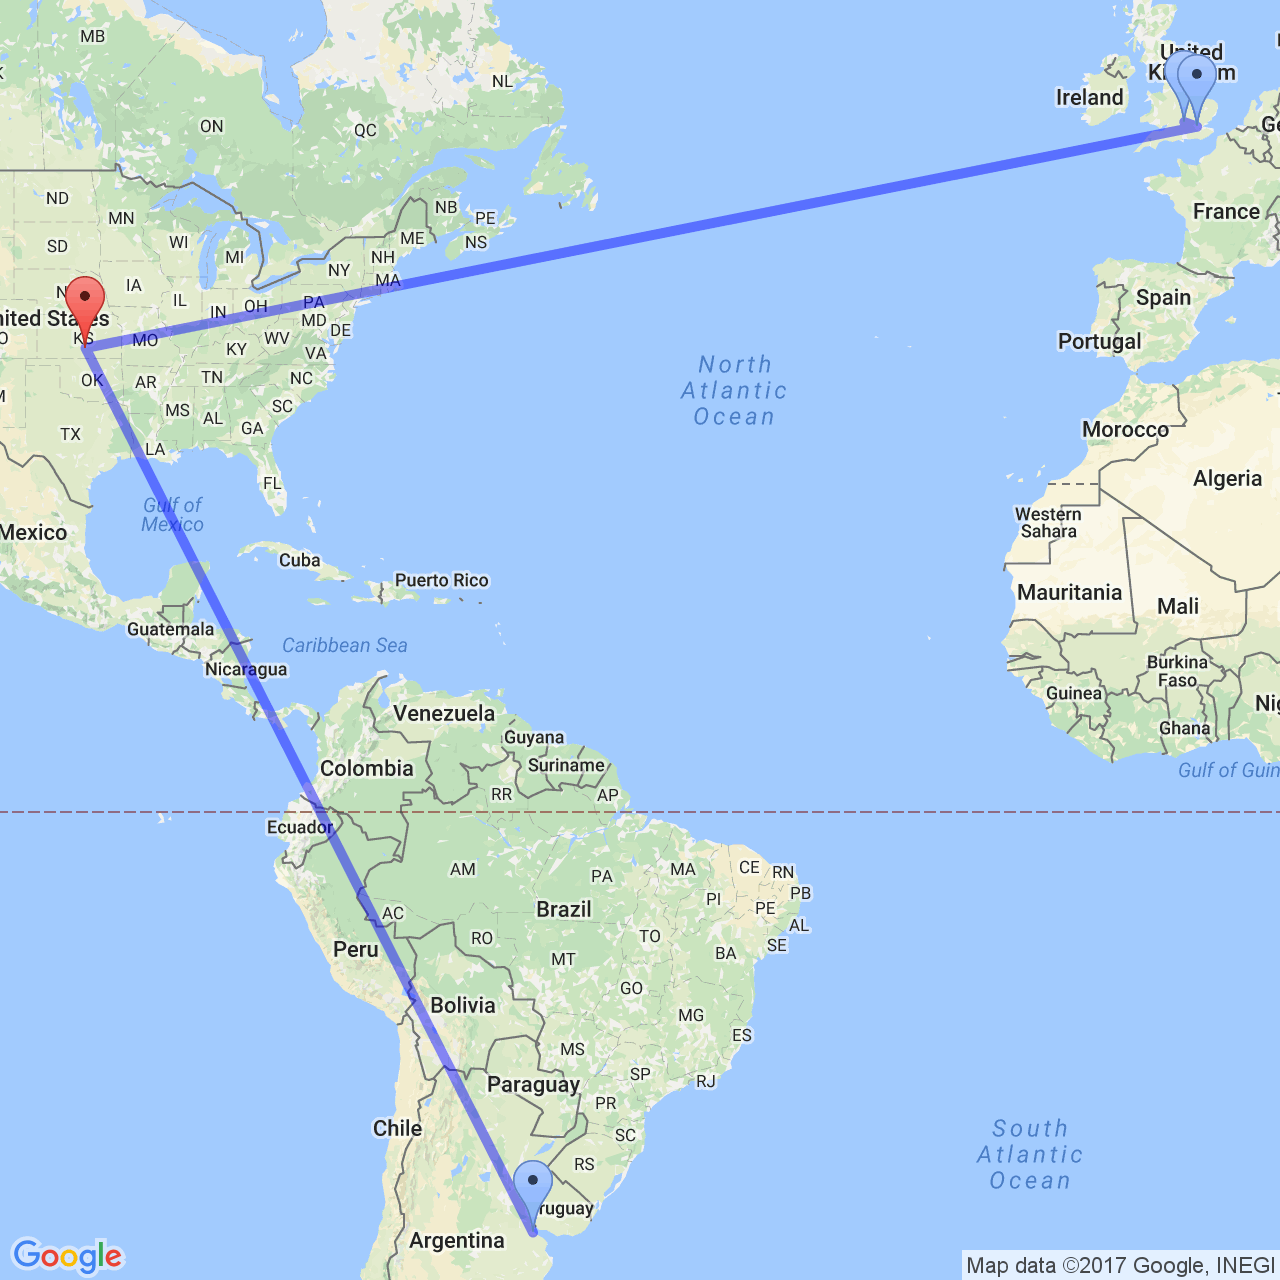
\includegraphics[width=0.55\textwidth]{modules/oxford_path_1}
 \label{fig:ruta_oxford_1}
\end{figure}

El servicio de geolocalizaci'on usado logra identificar la ruta desde Londres a Oxford pero no todos los puntos dentro de la Argentina, suponemos que la raz'on se
debe a que los proveedores de Argentina registran sus direcciones con ubicaciones en la ciudad de Buenos Aires mientras que los de Inglaterra en las ciudades
correspondientes.
\begin{figure}[H]
\centering
\caption{Ruta Londres-Oxford}
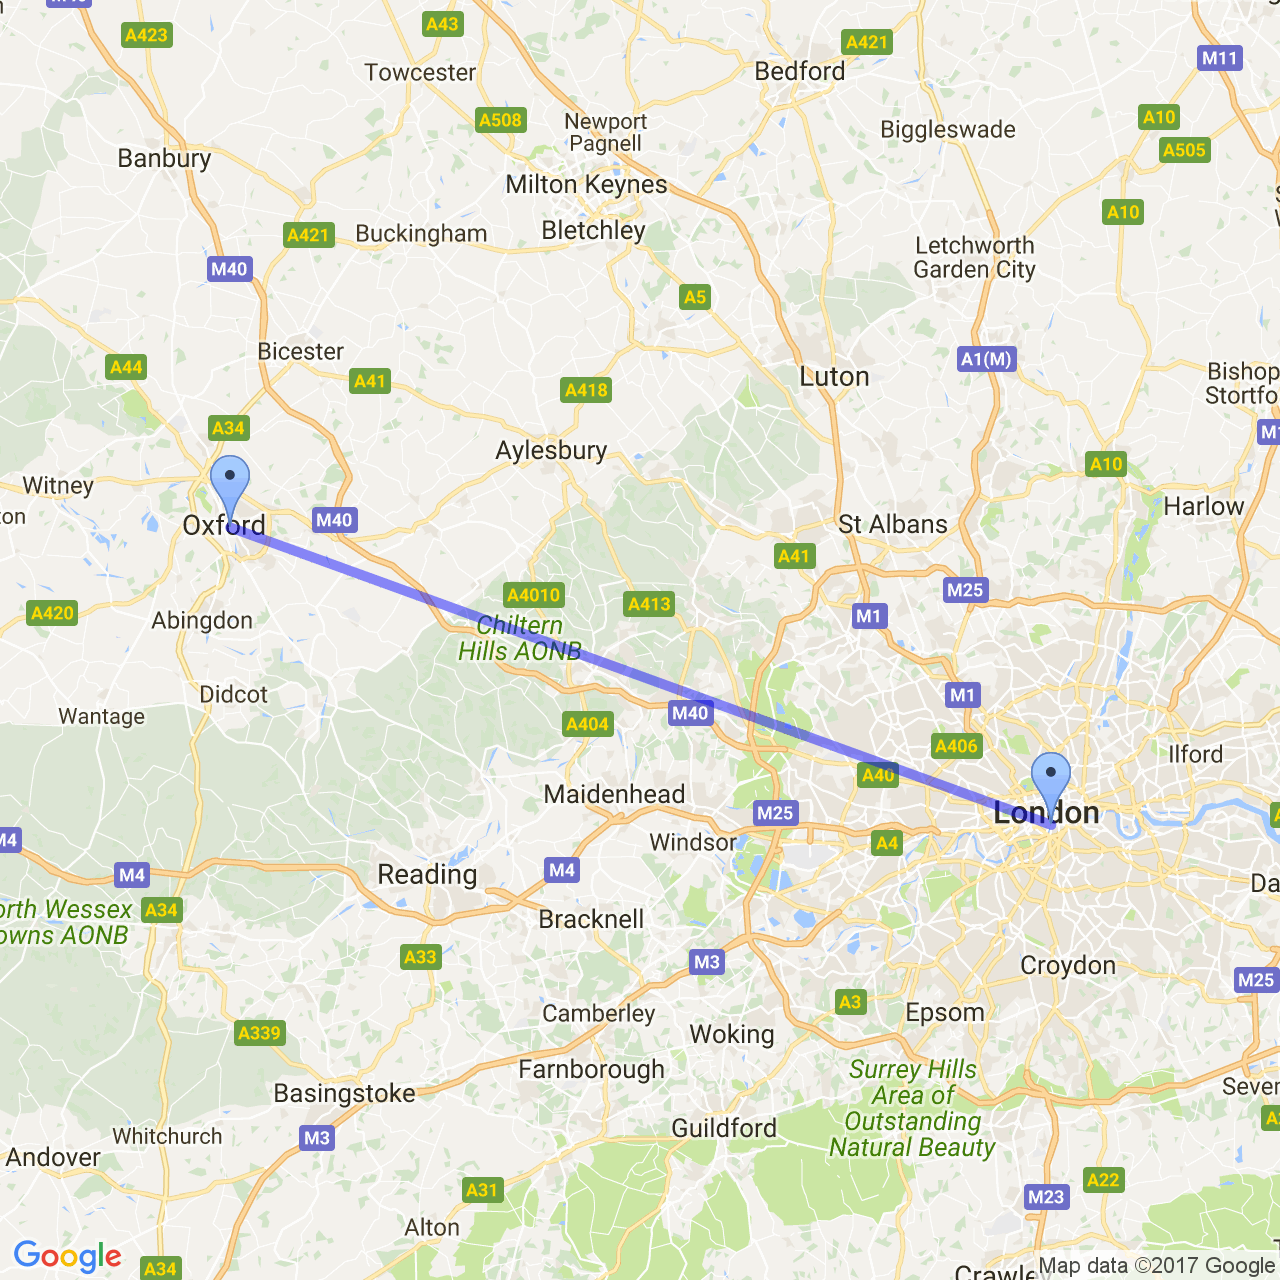
\includegraphics[width=0.55\textwidth]{modules/oxford_path_2}
 \label{fig:ruta_oxford_2}
\end{figure}
